\documentclass[8pt,a4paper,compress,handout]{beamer}

\usepackage{/home/siyer/lib/slides}

\title{Case Study: PageRank Algorithm}
\date{}

\begin{document}
\begin{frame}
\begin{flushright}
\tiny \textsc{An algorithm must be seen to be believed. \\ - Donald Knuth}
\end{flushright}
\titlepage
\end{frame}

\begin{frame}
\frametitle{Outline}
\tableofcontents
\end{frame}

\section{Random Surfer Model}
\begin{frame}[fragile]
\pause

The random surfer model is a simple model of the world-wide web (www) that has proven to be a particularly useful approach to understand some of its properties.

\bigskip

The www is modeled as a fixed set of pages, with each page containing a fixed set of links (called hyperlinks), and each link is a reference to some other page; such an abstraction is called a \textit{graph} in mathematics.

\bigskip

We are interested in what happens to a person (a random surfer) who randomly moves from page to page according to the \emph{90-10 rule}: 90\% of the time the random surfer clicks a random link on the current page (each chosen with equal probability) and 10\% of the time the random surfer goes directly to a random page by typing a page name into the address bar (all pages on the www are chosen with equal probability).
\end{frame}

\section{Input Format}
\begin{frame}[fragile]
An example of a tiny web of five pages and the file \lstinline{tiny.txt} that encodes it:

\begin{center}
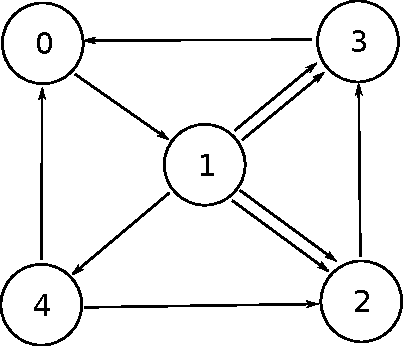
\includegraphics[scale=0.6]{figures/tiny_www.pdf}

\smallskip

\tiny A web of five pages
\end{center}

\begin{lstlisting}[language={}]
$ more tiny.txt
5
0 1
1 2 1 2
1 3 1 3
1 4
2 3
3 0
4 0 4 2
\end{lstlisting}
\end{frame}

\section{Transition Matrix}
\begin{frame}[fragile]
The transition matrix $P$ for a www with $N$ pages is an $N$-by-$N$ matrix such that the entry $P_{ij}$, i.e., the entry in row $i$ and column $j$, is the probability that the random surfer moves to page $j$ when on page $i$.

\bigskip

For example, a transition matrix for our tiny five-page web is:
\[
P = \begin{bmatrix}
0.02 & 0.92 & 0.02 & 0.02 & 0.02 \\
0.02 & 0.02 & 0.38 & 0.38 & 0.20 \\
0.02 & 0.02 & 0.02 & 0.92 & 0.02 \\
0.92 & 0.02 & 0.02 & 0.02 & 0.02 \\
0.47 & 0.02 & 0.47 & 0.02 & 0.02
\end{bmatrix}
\]
\end{frame}
\begin{frame}[fragile]
\begin{framed}
\tiny transition.py: Read links from standard input and write the corresponding transition matrix to standard output. First, process the input to count the outlinks from each page. Then apply the 90-10 rule to compute the transition matrix. Assume that there are no pages that have no outlinks in the input.
\end{framed}

\begin{lstlisting}[language=Python]
import stdarray
import stdio

n = stdio.readInt()
linkCounts = stdarray.create2D(n, n, 0)
outDegrees = stdarray.create1D(n, 0)
while not stdio.isEmpty():
    i = stdio.readInt()
    j = stdio.readInt()
    outDegrees[i] += 1
    linkCounts[i][j] += 1
stdio.writeln(str(n) + ' ' + str(n))
for i in range(n):
    for j in range(n):
        p = (.90 * linkCounts[i][j] / outDegrees[i]) + (.10 / n)
        stdio.writef('%8.5f', p)
    stdio.writeln()
\end{lstlisting}

\begin{lstlisting}[language={}]
$ python transition.py < tiny.txt
5 5
 0.02000 0.92000 0.02000 0.02000 0.02000
 0.02000 0.02000 0.38000 0.38000 0.20000
 0.02000 0.02000 0.02000 0.92000 0.02000
 0.92000 0.02000 0.02000 0.02000 0.02000
 0.47000 0.02000 0.47000 0.02000 0.02000
\end{lstlisting}
\end{frame}

\section{Simulating a Random Surfer}
\begin{frame}[fragile]
\begin{framed}
\tiny randomsurfer.py: Accept an integer $moves$ as a command-line argument. Read a transition matrix from standard input. Perform $moves$ moves as prescribed by the transition matrix, and write to standard output the relative frequency of hitting each page, i.e., its page rank.
\end{framed}

\begin{lstlisting}[language=Python]
import random
import stdarray
import stdio
import sys

moves = int(sys.argv[1])
n = stdio.readInt()
stdio.readInt()
p = stdarray.create2D(n, n, 0.0)
for i in range(n):
    for j in range(n):
        p[i][j] = stdio.readFloat()
hits = stdarray.create1D(n, 0)
page = 0
for i in range(moves):
    r = random.random()
    total = 0.0
    for j in range(0, n):
        total += p[page][j]
        if r < total:
            page = j
            break
    hits[page] += 1
for v in hits:
    stdio.writef("%8.5f", 1.0 * v / moves)
stdio.writeln()
\end{lstlisting}
\end{frame}

\begin{frame}[fragile]
\begin{lstlisting}[language={}]
$ python transition.py < tiny.txt | python randomsurfer.py 100
 0.26000 0.27000 0.18000 0.26000 0.03000
$ python transition.py < tiny.txt | python randomsurfer.py 10000
 0.27410 0.26500 0.14570 0.24890 0.06630
$ python transition.py < tiny.txt | python randomsurfer.py 10000000
 0.27308 0.26568 0.14616 0.24719 0.06789
\end{lstlisting}
\end{frame}

\section{Markov Chain}
\begin{frame}[fragile]
A \emph{Markov chain} is a random process that describes behavior similar to the random surfer. 

\bigskip

A remarkable and useful property of Markov chains is that of \emph{mixing}, which states that the random surfer could start anywhere, since the probability that the surfer eventually winds up on any particular page is the same for all starting pages.

\bigskip

\emph{Page rank} is the probability that the random surfer lands on a page. 

\bigskip

Because of the mixing phenomenon, increasing the number of iterations in the simulation of the random surfer gives increasingly accurate estimates of page ranks.
\end{frame}

\begin{frame}[fragile]
Using the \emph{power method} we can obtain the probability that the random surfer will move from page $i$ to page $j$ in two moves by multiplying the transition matrix $P$ by itself. 

\bigskip

In general, the probability that the random surfer will move from page $i$ to page $j$ in $t$ moves is obtained by computing $P^t$. 

\bigskip 

But matrix-matrix multiplication is expensive. Fortunately, because of the mixing property, we can make do with relatively inexpensive vector-matrix multiplications. 
\end{frame}

\begin{frame}[fragile]
For example, with our tiny web, if we start with the vector 
\[
\begin{bmatrix}
1.0 & 0.0 & 0.0 & 0.0 & 0.0
\end{bmatrix}
\]
specifying that the random surfer starts on page 0, multiplying the vector by the transition matrix $P$ gives the vector 
\[
\begin{bmatrix}
0.02 & 0.92 & 0.02 & 0.02 & 0.02
\end{bmatrix}
\]
specifying the probabilities that the surfer winds up on each of the pages after one step. 

\bigskip

Now, multiplying the above vector by the transition matrix $P$ gives the vector
\[
\begin{bmatrix}
0.05 & 0.04 & 0.36 & 0.37 & 0.19
\end{bmatrix}
\]
which contains the probabilities that the surfer winds up on each of the pages after two steps. 

\bigskip

The vector giving the probabilities that the random surfer is at each page after $t$ steps is the product of the corresponding vector for $t-1$ steps and the transition matrix $P$. 
\end{frame}

\begin{frame}[fragile]
\begin{framed}
\tiny markov.py: Accept integer $moves$ from the command-line, and read a transition matrix from standard input. Compute the probabilities that a
random surfer lands on each page (page ranks) after $moves$ matrix-vector multiplications, and write the page ranks to standard output.
\end{framed}

\begin{lstlisting}[language=Python]
import stdarray
import stdio
import sys

moves = int(sys.argv[1])
n = stdio.readInt()
stdio.readInt()
probs = stdarray.create2D(n, n, 0.0)
for i in range(n):
    for j in range(n):
        probs[i][j] = stdio.readFloat()
ranks = stdarray.create1D(n, 0.0)
ranks[0] = 1.0
for i in range(moves):
    newRanks = stdarray.create1D(n, 0.0)
    for j in range(n):
        for k in range(n):
            newRanks[j] += ranks[k] * probs[k][j]
    ranks = newRanks
for rank in ranks:
    stdio.writef("%8.5f", rank)
stdio.writeln()
\end{lstlisting}

\begin{lstlisting}[language={}]
$ python transition.py < tiny.txt | python markov.py 20
 0.27245 0.26515 0.14669 0.24764 0.06806
$ python transition.py < tiny.txt | python markov.py 40
 0.27303 0.26573 0.14618 0.24723 0.06783
\end{lstlisting}
\end{frame}
\end{document}
